\documentclass[11pt]{article}

% Packages for Figures:
\ifx\pdftexversion\undefined
    \usepackage[dvips]{graphicx}
\else
    \usepackage[pdftex]{graphicx}
    \usepackage{epstopdf}
    \epstopdfsetup{suffix=}
\fi

% Packages for displaying code:
\usepackage{listings}
\usepackage{textcomp}
\usepackage{color}

% Color settings used in the code below:
\definecolor{dkgreen}{rgb}{0,0.6,0}
\definecolor{gray}{rgb}{0.5,0.5,0.5}
\definecolor{mauve}{rgb}{0.58,0,0.82}

% Settings for the formatting of the code on display:
\lstset{frame=tb,
  language=R,
  aboveskip=3mm,
  belowskip=3mm,
  showstringspaces=false,
  columns=flexible,
  basicstyle={\small\ttfamily},
  numbers=none,
  numberstyle=\tiny\color{gray},
  keywordstyle=\color{blue},
  commentstyle=\color{dkgreen},
  stringstyle=\color{mauve},
  breaklines=true,
  breakatwhitespace=true,
  tabsize=3
}


\begin{document}


\section{Introduction}

This document displays a table in Section \ref{sec:tab}, 
an equation in Section \ref{sec:eqn}, 
and some code that generates a figure in Section \ref{sec:fig}.


\section{A Table} \label{sec:tab}

This is my document.

In Table \ref{tab:summary}, there are some numbers.

\begin{table}[ht]
\centering
\begin{tabular}{rlrr}
  \hline
 & Statistic & Variable 1 & Variable 2 \\
  \hline
  1 & Min. & 0.19 & 0.08 \\
  2 & Mean & 0.70 & 0.10 \\
  3 & S.D. & 0.18 & 0.01 \\
  4 & Max. & 1.09 & 0.13 \\
   \hline
\end{tabular}
\caption{Summary of Numeric Variables}
\label{tab:summary}
\end{table}


\section{An Equation} \label{sec:eqn}

This is an inline equation: $y_i = \beta_0 + \beta_1 x_i + \epsilon_i$. 

\noindent It is shown again using the \texttt{equation} environment 
 in Equation (\ref{eqn:reg}). In this format, you can refer to 
Equation (\ref{eqn:reg}) by number, in case you have many equations. 

\begin{equation} \label{eqn:reg}
y_i = \beta_0 + \beta_1 x_i + \epsilon_i
\end{equation}


\section{Histogram of a Randomly Generated Variable} \label{sec:fig}

We ran the following commands in R.

\begin{lstlisting}[language=R]
R> # Generate a random variable.
    epsilon <- rnorm(1000)
    
    # Plot a histogram.
    fig_ext <- 'eps'
    fig_dir <- 'Figures'
    fig_file_name <- sprintf('name_of_figure.%s', fig_ext)
    out_file_name <- sprintf('%s/%s', fig_dir, fig_file_name)
    
    setEPS()
    postscript(out_file_name)
    
    hist(epsilon, col = 'blue')
    
    dev.off()
    
\end{lstlisting}


The histogram in Figure \ref{fig:example} shows the result of these commands.

\begin{figure}[h]
\centering
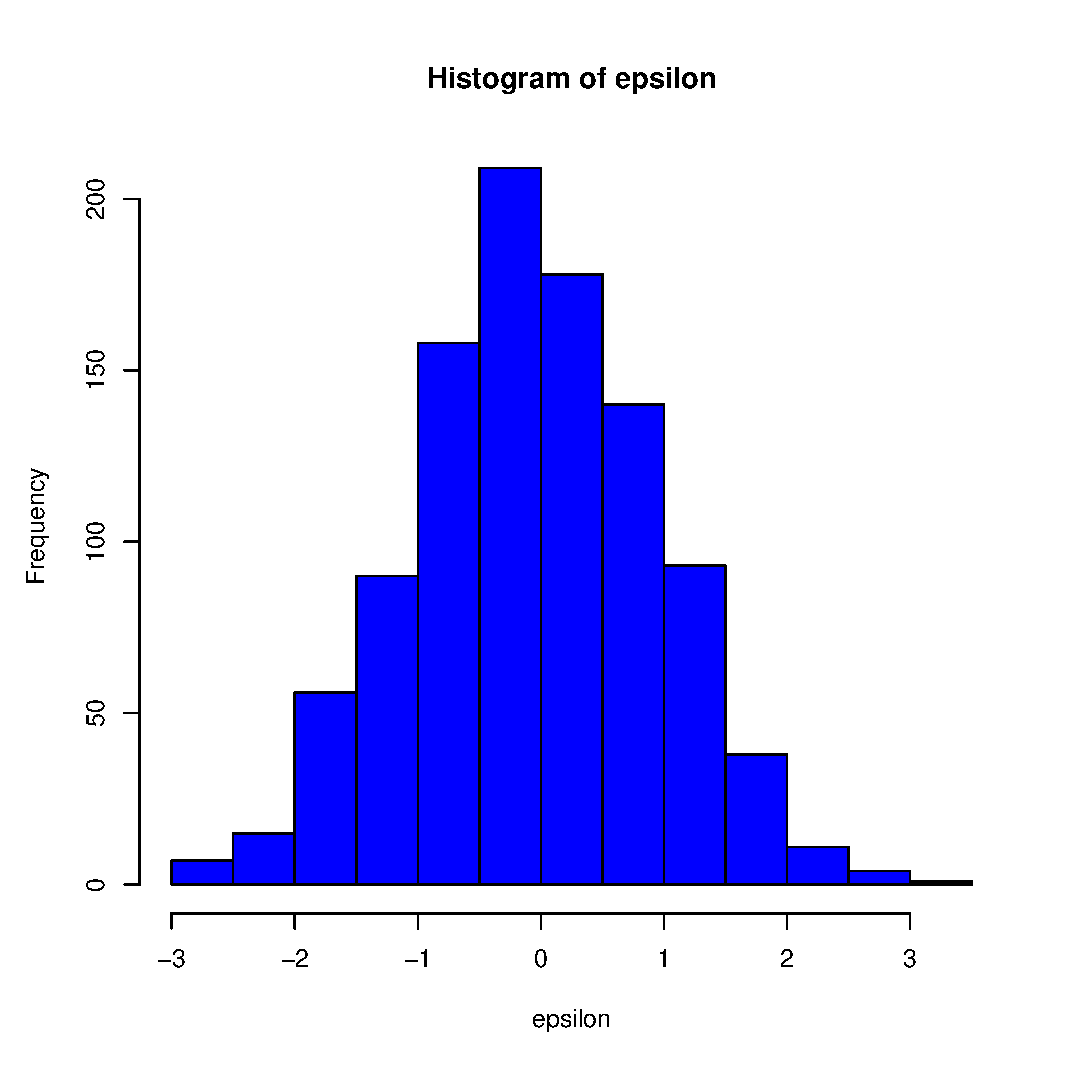
\includegraphics[width=\textwidth]{Figures/name_of_figure.eps}
\caption{Caption Goes Here}
\label{fig:example}
\end{figure}


\end{document}
